\documentclass{article}

% various packages and settings {{{

% math packages
\usepackage{amsmath, amsfonts, mathtools}

% other important packages (should stay on top)
\usepackage{graphics, multicol, xcolor}

% change to German
\usepackage[german]{babel}

% utf8 characters
\usepackage[utf8]{inputenc}

% font
\usepackage[scaled]{helvet}
\renewcommand{\familydefault}{\sfdefault}
\usepackage[]{fontspec}

% fontsize
\usepackage[12pt]{extsizes}

% no paragraph indents
\setlength{\parindent}{0pt}

% better hyphenation
\usepackage[final]{microtype}
\usepackage{csquotes}

% import line spacing
\usepackage{setspace}

% page format
\usepackage{geometry}
\geometry{
    a4paper,
    left=25mm,
    right=25mm,
    top=15mm,
    bottom=25mm
}

% colorful boxes
\usepackage{mdframed}

\setcounter{secnumdepth}{0} % no section numbering
% }}}

% custom commands {{{
\usepackage{environ}

% define custom formula environment
\NewEnviron{formulas}{
    \vspace{-2.5em}
    \Large
    \begin{align*}
        \BODY
    \end{align*}
    \normalsize
}

% same formula env, but with red border
\NewEnviron{Formulas}{
    \begin{mdframed}[linecolor=red]
        \vspace{-2.5em}
        \Large
        \begin{align*}
            \BODY
        \end{align*}
        \normalsize
    \end{mdframed}
}

% normal-sized text inside the formulas
\newcommand{\normaltext}[1]{
    \normalsize\text{#1}\Large
}

% }}}

\begin{document}

\addtocounter{page}{-2}
\setstretch{1.5}

\title{Mathematik}
\date{\today}
\maketitle

\thispagestyle{empty}

\clearpage

\tableofcontents

\thispagestyle{empty}

\clearpage

% ------------ Vektoren, Geraden, Ebenen, Abstände im Raum ------------ %
\section{Vektoren}

\graphicspath{ {./images/} }

\subsection{Vektoren}

Ein Vektor beschreibt eine Strecke mit Richtung zwischen 2 Punkten im Raum.
Ein Vektor kann von jedem Ort im Raum ausgehen.und hat immer einen Start- und Endpunkt. 
Jeder Punkt im Raum lässt sich als Vektor vom Ursprung $O$ zu den Koordinaten des Punktes
darstellen.

\begin{equation}
    P (1, 3, 2) \rightarrow \overrightarrow{OP} = \begin{bmatrix}
        1 \\
        3 \\
        2
    \end{bmatrix}
    \qquad A (1, 2, 2) \; B (4, 3, 1) \rightarrow \overrightarrow{AB} = \begin{bmatrix}
        3 \\
        1 \\
        -1
    \end{bmatrix}
\end{equation}

\subsection{Vektorrechnung}

\subsubsection{Länge eines Vektor}

Die Länge eines Vektors ergibt sich aus dem Satz des Pythagoras.
Betragsstriche um einen Vektor bedeuten, dass dessen Länge gemeint ist.

\begin{equation}
    \overrightarrow{AB} = \begin{bmatrix}
        3 \\
        1 \\
        -1
    \end{bmatrix}
    \qquad | \overrightarrow{AB} | = \sqrt{3^2 + 1^2 + (-1)^2} = \sqrt{11}
\end{equation}

\subsubsection{Skalarprodukt}

Das Skalarprodukt ist die Summe der Produkte der einzelnen Vektorelemente.
Das Ergebnis ist eine relle Zahl.

\begin{equation}
    \begin{bmatrix}
        3 \\
        1 \\
        -1
    \end{bmatrix} \cdot
    \begin{bmatrix}
        2 \\
        0 \\
        -1
    \end{bmatrix} = 3 \cdot 2 + 1 \cdot 0 + -1 \cdot -1 = 7
\end{equation}

\subsubsection{Kreuzprodukt}

Das Kreuzprodukt zweier Vektoren ergibt einen dritten Vektor der orthogonal
zu beiden anderen ist.

\begin{equation}
    \vec{a} \times \vec{b} =
    \begin{bmatrix}
        a_1 \\
        a_2 \\
        a_3
    \end{bmatrix} \times
    \begin{bmatrix}
        b_1 \\
        b_2 \\
        b_3
    \end{bmatrix} =
    \begin{bmatrix}
        a_2 b_3 - a_3 b_2 \\
        a_3 b_1 - a_1 b_3 \\
        a_1 b_2 - a_2 b_1
    \end{bmatrix}
\end{equation}

% 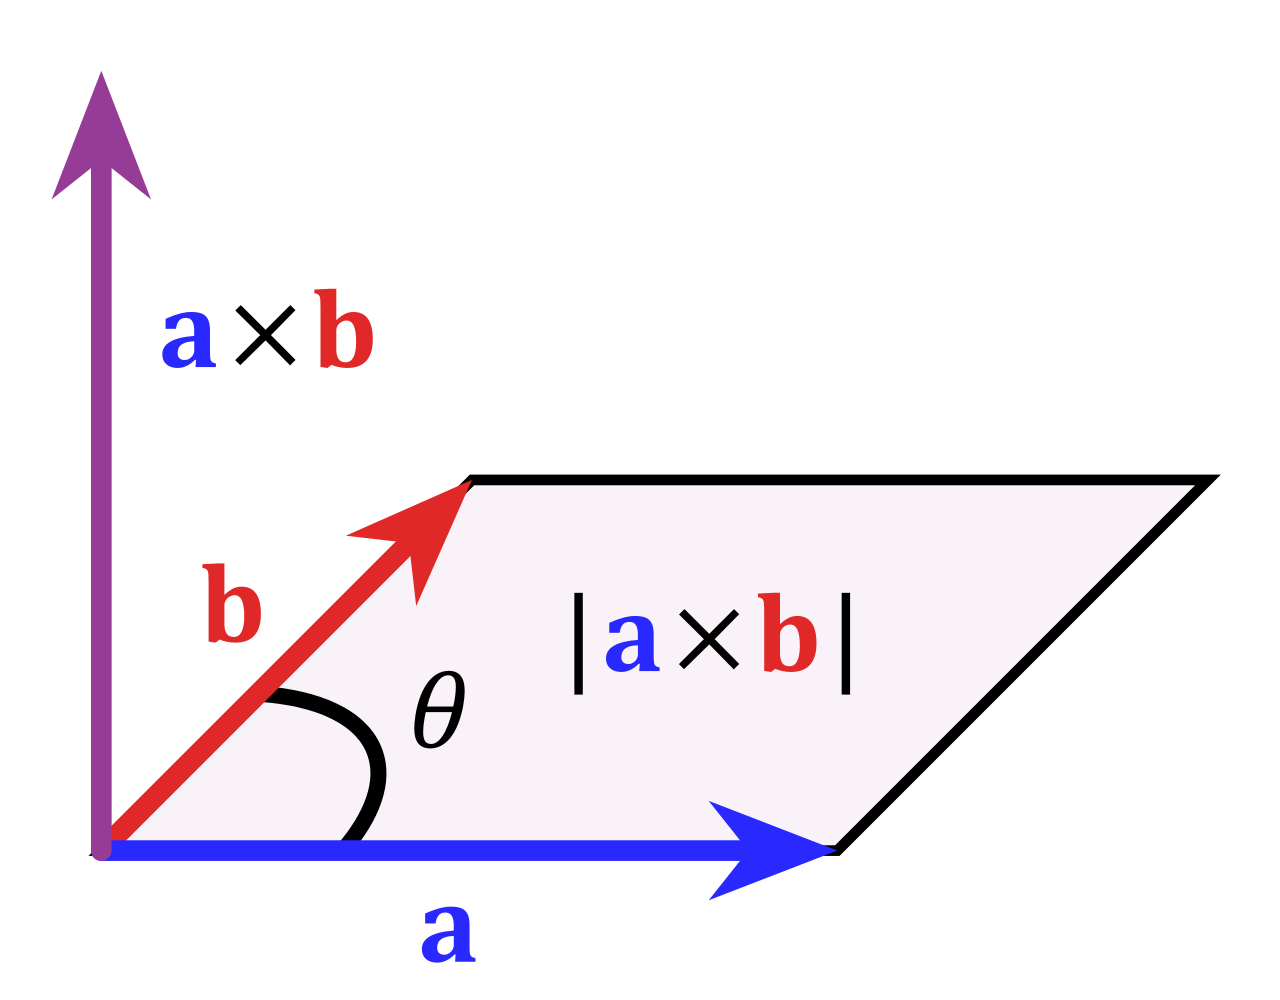
\includegraphics{cross-p}

\begin{equation}
    \begin{bmatrix}
        3 \\
        1 \\
        -1
    \end{bmatrix} \times
    \begin{bmatrix}
        2 \\
        0 \\
        -1
    \end{bmatrix} =
    \begin{bmatrix}
        1 \cdot (-1) - (-1) \cdot 0 \\
        (-1) \cdot 2 - 3 \cdot (-1) \\
        3 \cdot 0 - 1 \cdot 2
    \end{bmatrix} =
    \begin{bmatrix}
        -1 \\
        1 \\
        -2
    \end{bmatrix}
\end{equation}


\end{document}
